% article example for classicthesis.sty
\documentclass[10pt,a4paper]{article} % KOMA-Script article scrartcl
\usepackage{lipsum}     %lorem ipsum text
\usepackage{titlesec}   %Section settings
\usepackage{titling}    %Title settings
\usepackage[margin=10em]{geometry}  %Adjusting margins
\usepackage{setspace}
\usepackage{listings}
\usepackage{amsmath}    %Display equations options
\usepackage{amssymb}    %More symbols
\usepackage{xcolor}     %Color settings
\usepackage{pagecolor}
\usepackage{mdframed}
\usepackage[spanish]{babel}
\usepackage[utf8]{inputenc}
\usepackage{longtable}
\usepackage{multicol}
\usepackage{graphicx}
\graphicspath{ {./Images/} }
\setlength{\columnsep}{1cm}

% ====| color de la pagina y del fondo |==== %
\pagecolor{white}
\color{black}



\begin{document}
    %========================{TITLE}====================%
    \title{\rmfamily\normalfont\spacedallcaps{ Laboratorio 2 : Forensics }}
    \author{\spacedlowsmallcaps{Rodrigo Castillo}}
    \date{\today} 
    
    \maketitle
     

    %=======================NOTES GOES HERE===================%
        \section{3 reasons that justify to do a Malware Analysis}
            \subsection{Primera razón}
                La primera razon por la cuál alguien querría analizar un malware es
                para buscar a sus creadores, pues muchos ataques informáticos son
                catastróficos para las empresas y por esta razón es bueno buscar a sus
                culpables

            \subsection{Segunda razón}
                Para dimensionar el daño potencial que pueda tener un archivo malicioso
                en un computador : Muchas veces nosotros descargamos contenido del cuál
                no sabemos su procedencia, por lo tanto, es bueno poder analizar que
                acciones está teniendo este contenido en nuestros dispositivos y de
                esta manera poder hacer un balance para saber si este contenido nos
                beneficia o nos perjudica.

            \subsection{Tercera razón}
                Para entender el Malware, entender el malware puede prevenirnos de
                futuros ataques informáticos en muchas ocaciones, nos puede enseñar
                como prevenirlo y en un ambiente de seguridad ofensiva , como
                ejecutarlo.
                \\ Además de todo lo anterior, entender el malware puede ser facinante
                y puede contribuir con otras diciplinas de la informática, con esto,
                construir herramientas que nos puedan beneifciar en un futuro.

        \section{Tipos de malware}
            \subsection{Backdoor}
                Un Backdoor(puerta trasera) es un programa o una brecha de
                seguridad que permite al
                atacante conectarse al dispositivo cada vez que el lo indique ,
                generalmente se usan generando software vulnerable de exprofeso
                o instalando scripts que permiten hacer eso. 
                \\ 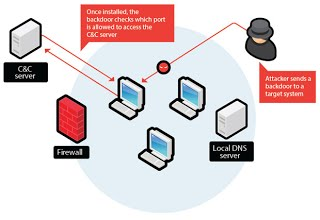
\includegraphics[width=0.8\linewidth]{backdoor.jpg}
                \\ 

            \subsection{Botnet}
                Una botnet es un programa que permite al atacante obtener el
                acceso de varias máquinas que no son suyas , esto puede tener
                varios fines, como hacer ataques DDOS , minar criptomonedas ,
                etc , las botnet siempre intentan adueñarse de la mayor
                cantidad de máquinas posible.
                \\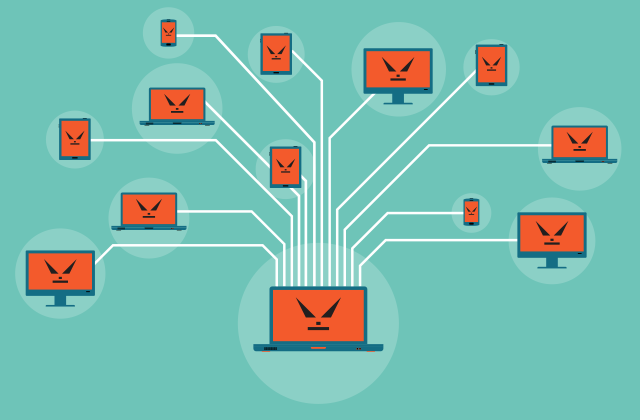
\includegraphics[width=0.8\linewidth]{botnet.jpg}
                \\ 

            \subsection{Downloader}
                Los Downloader son programas que descargan e
                instalan nuevas versiones de programas maliciosos , como
                troyanos y adware en las computadoras de las víctimas. 
                Estos programas se ejecutan automáticamente cuando
                se inicia el sistema operativo.
                \\
\includegraphics[width=0.8\linewidth]{downloader.png}
                \\ 

            \subsection{information stealing malware}
                hay muchas manifestaciones de malware para robar información,
                pero se clasifican todos los programas maliciosos que están
                diseñados para mandar información del interés del atacante sin
                el consentimiento de la víctima .
                \\ 
                \\ 
\includegraphics[width=0.8\linewidth]{information.jpg}
                \\ 

            \subsection{Launcher}
                un Launcher es un tipo de malware que ejecuta otro malware.

            \subsection{Rootkit}
                Un rootkit es una brecha de seguridad que permite al atacante
                elevar los privilegios a privilegios no autorizados, pueden ser
                programas vulnerables del sistema operativo que se ejecutan con
                permisos de administrador o explotan la funcion setuid, pueden
                ser implantados por el atacante como estar instalados por el
                dueño de la maquina. Un ejemplo de un rootkit es la aplicación de Zoom.

            \subsection{Scareware}
                Un Scareware es un programa que simula ser un antivirus o un
                servicio de seguridad, le advirte al usuario que la seguridad
                de su equipo esta en riesgo por alguna razon y luego le pide
                sus credenciales para protegerlo. 
                \\ 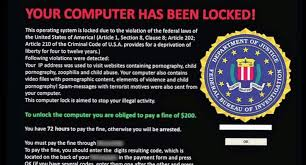
\includegraphics[width=1.2\linewidth]{scareware.jpeg}
                \\ 

            \subsection{Spam Sending Malware}
                Un malware de spam es un tipo de malware que infecta a un
                dispositivo o se roba sus credenciales, y a travéz de esta las
                usa para mandar publicidad  , hay varios ejemplos de este.
                
                \\ 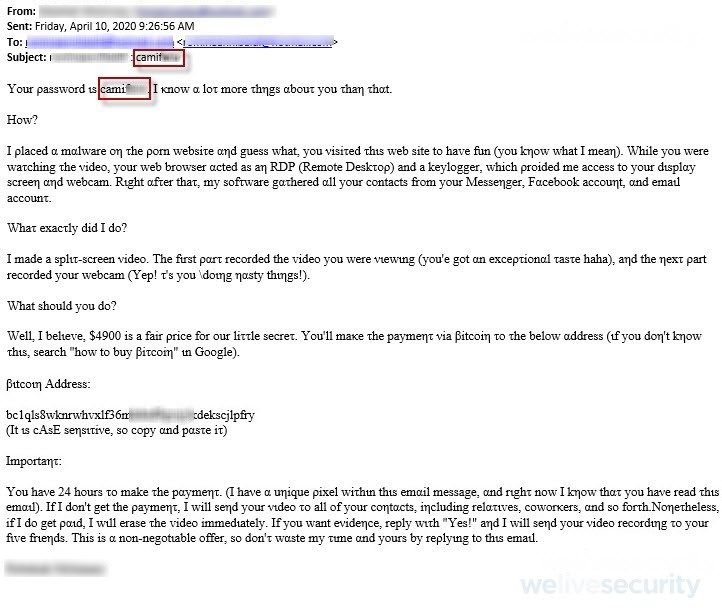
\includegraphics[width=0.8\linewidth]{scam.jpeg}
                \\ 

            \subsection{Virus}
                un virus informático es un programa malicioso que en sus
                funciones intenta replicarse en otros dispositivos, ya sea por
                correos, a travez de la red, aplicaciones, etc.

            \subsection{Worm}
                un gusano informático es un tipo de virus , un programa
                malicioso que una vez
                infecta un dispositivo, intenta propagarse a los dispositivos
                que se encuentren en su red. 
                \\ 


                
        \section{Malware analysis techniques}
            \subsection{Basic Static Analisis}
                \subsection{what this analysis inspect}
                    consiste en inspeccionar facciones generales del malware,
                    como su hash(caracterización) o la cantidad de elementos
                    que tiene, no se puede saber mucho de su funcionamiento
                    pero tampoco requiere mucho trabajo pues existen
                    herramientas como virustotal que hacen eso automáticamente.
                \subsubsection{what is the product of this analysis}
                    se puede identificar el malware

            \subsection{Basic Dynamic Analysis}
                \subsubsection{What this analysis inspects}
                    consiste en ejecutar un binario malicioso en un entorno
                    controlado llamado sandbox con eso, se puede saber el daño
                    potencial de este binario.

                \subsubsection{What is the product of this analysis}
                    se puede visualizar el funcionamiento del malware sin
                    necesidad de exponer una máquina real.

            \subsection{Advanced Static Analysis}
                \subsubsection{What this analysis inspects}
                    Éste analisis mira el código assembly de un binario o el
                    código fuente de un lenguaje interpretado, lo que busca es
                    reconstruir el codigo fuente del programa, con eso es
                    posible entender el funcionamiento de un este. Para
                    esto, se hace uso de una herramienta llamada un
                    dissasembler, que reconstruye el código assembly de un
                    programa sin necesidad de ejecutarlo.

                \subsubsection{What is the product of this analysis}
                    Haciendo disassembly debidamente se puede entender todo el
                    funcionamiento de un programa sin necesidad de ejecutarlo,
                    sin embargo, hacer disassebly debidamente es un proceso muy
                    complicado que requiere mucha practica , experiencia y dedicación.

            \subsection{Advanced dynamyc annalysis}
                 \subsubsection{What this analysis inspects}
                    Este analisis analiza el funcionamiento del programa paso
                    por paso, haciendo debugging se puede reconstruir el código
                    y tener un panorama bastante amplio del funcionamiento del
                    virus , un debugger es una herramienta con la cual se puede
                    ejecutar el programa paso a paso y analizar cada paso, se
                    pueden poner breakpoints, se pueden modificar los registros
                    del programa, se puede forzar el programa a tomar otros
                    flujos de ejecución...etc .

                 \subsubsection{What is the product of this analysis}
                    se puede entender casi perfectamente la manera en la que el
                    virus fue construído y su funcionamiento .

        \section{Diferencia entre Host Based Signatures y Antivirus Based Signatures}
           \subsection{Host Based Signatures}
                Las firmas basadas en host, son firmas que analizan los
                binarios fijandose en el funcionamiento de estos para decir si
                son malware o no, si un programa pide muchos permisos, si se
                conecta a ips poco confiables, es mas probable que sean malware.
                
           \subsection{Antivirus Based Signatures}
                Las firmas basadas en antivirus son firmas que usan modelos de
                machine learning para detectar si algo es malware , entrenados
                con lo que ellas conocen que es malware, sin embargo, estas no
                son tan eficaces como las firmas basadas en características
                pues, los atacantes usan distintas técnicas de cifrado de
                malware con el fin de evitar estos reconocimientos de machine
                learning.
               
                
   
                
                
                
                
        \section{Download a file from from Malware Zoo
        (https://github.com/ytisf/theZoo) and upload it to VirusTotal.com.
        Review the host-based, antivirus, and network-based signatures reported
        by VirusTotal.com. What is the difference between host-based signatures
        and antivirus signatures? }

            \subsection{Selección del malware}
                con propósitos del análisis, me dispuse a buscar un archivo
                binario de malware el cuál podré inspeccionar, en este curso,
                elegí el archivo Trojan.Alien\_Spy : 

                \\ 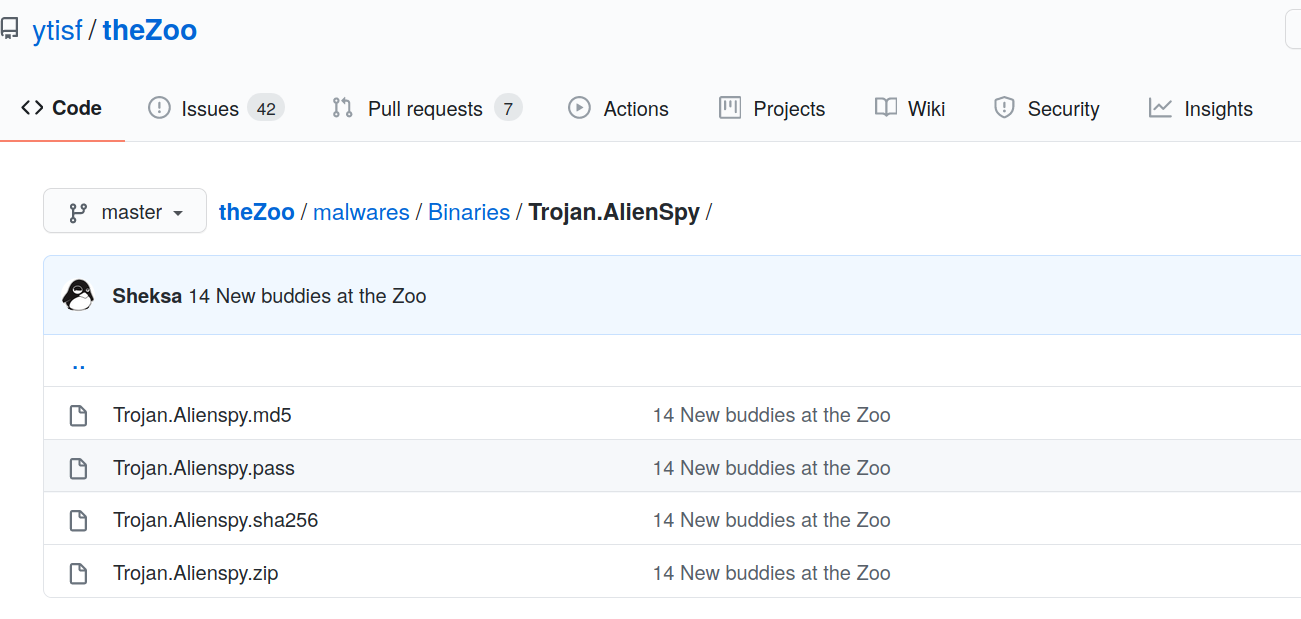
\includegraphics[width=0.5\linewidth]{alien_spy.png}}
                \\ el cual contiene un archivo comprimido con su binario.\\

                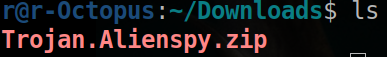
\includegraphics[width=0.5\linewidth]{trojanzip.png}
                \\una vez descomprimido el archivo, obtenemos estos archivos
                .jar que hacen referencia a que este es un malware escrito en
                java  

                \\ 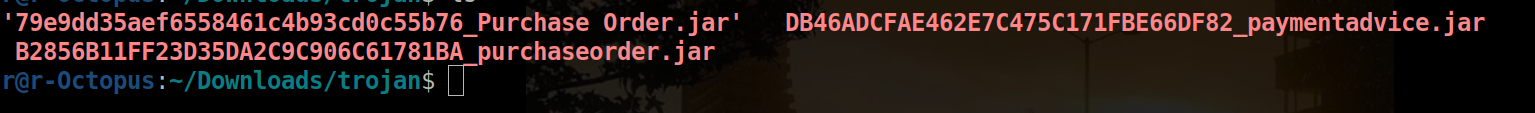
\includegraphics[width=0.5\linewidth]{filestrojan.png}

            \subsection{Analisis  estatico:}
                Para ejecutar el analisis  estático vamos a usar el servicio de
                virustotal, por lo que subiremos el archivo zip a virustotal.

                \subsubsection{Analizando el malware como archivo zip con
                antivirus conocidos(antivirus based signatures)}

                    Virustotal es un servicio que usa diferentes servicios para
                    ejecutar el analisis  estatico de un malware, sin embargo, solo 3
                    de 61 de sus servicios detectaron que era un malware.
                    \\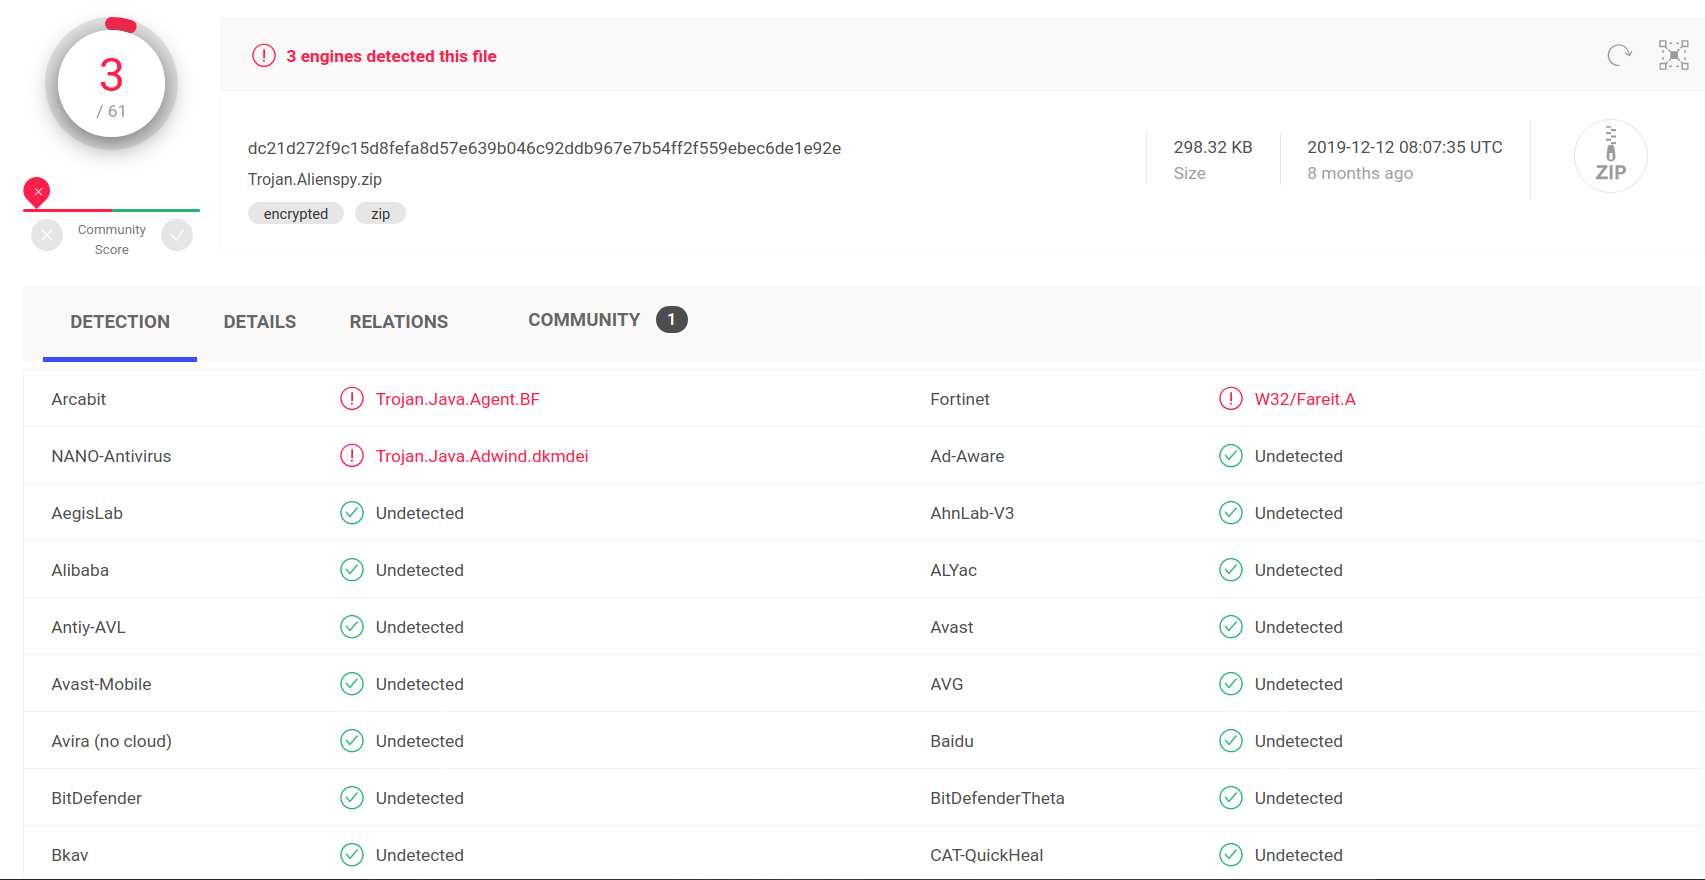
\includegraphics[width=0.5\linewidth]{virustotal_antivirus.png}

                \subsubsection{Analizando el virus como archivo zip con otras propiedades (host
                based signatures and network based signatures)}
                    propiedades basicas del virus 
                    \\ 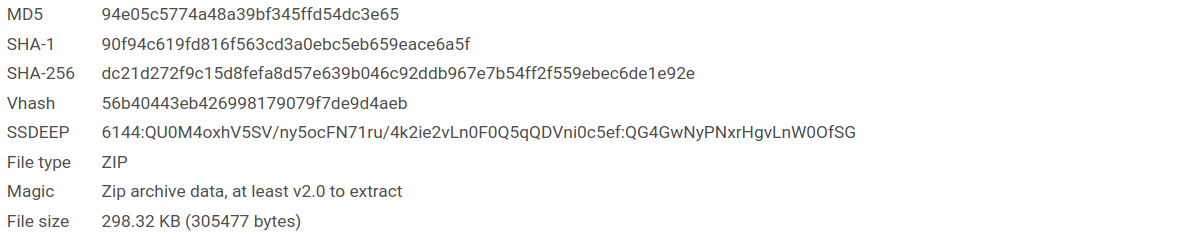
\includegraphics[width=0.5\linewidth]{propiedadesbasicas.png}
                    \\ 
                    \\ Estas propiedades hacen referencia a los hash del virus,
                    a las carácterísticas del virus que identifican al archivo.
                    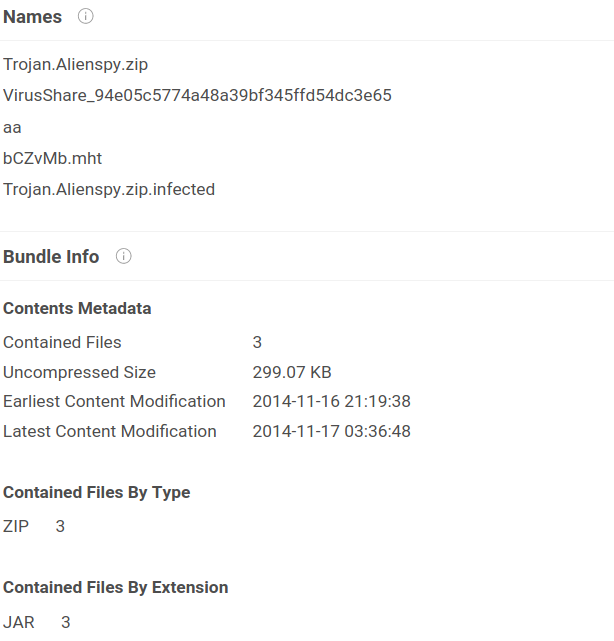
\includegraphics[width=0.5\linewidth]{otraspropiedades.png}
                    \\ 
                    el antivirus analiza los archivos que hay dentro del
                    documento comprimido y retorna que tiene 3 archivos
                    comprimidos con extension .jar, por lo que ahora
                    procederemos a analizar los archivos jar individualmente.

                \subsubsection{Analizando los archivos jar con antivirus
                (antivirus based signatures)}
                    ya ejecutando el analisis con el primer binario en java, podemos
                    ver que 40 de los 61 antivirus detectan que es un troyano: 

                    \\ 
                    \\ 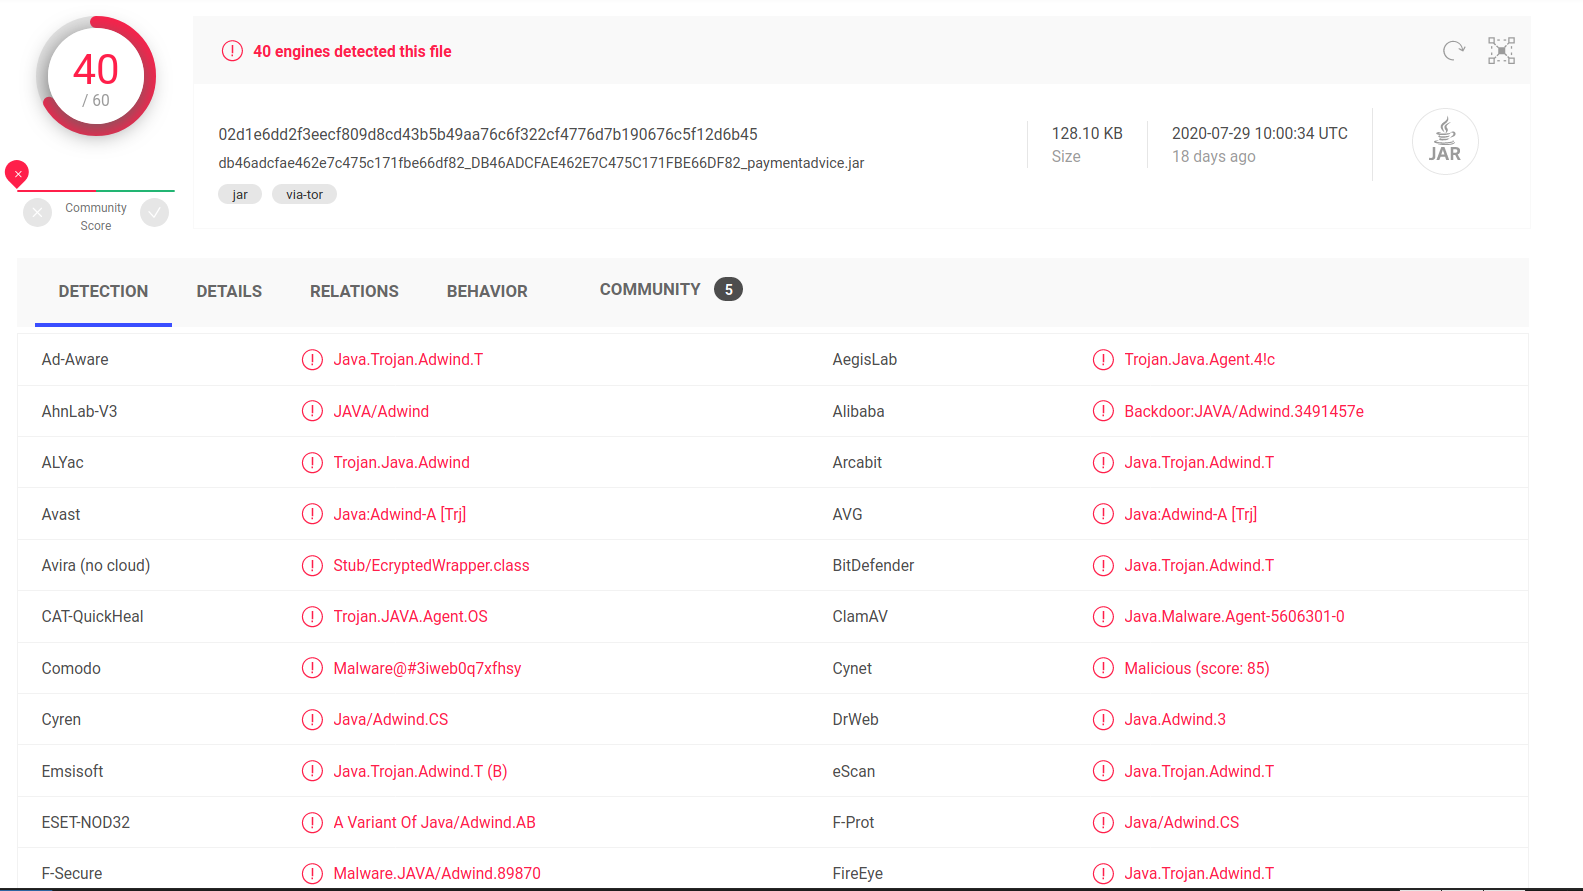
\includegraphics[width=0.5\linewidth]{payment.png}

                    \\
                    \\ ejecutando el analisis con el segundo binario 41 de los 60 antivirus lo reconocen

                    \\ 
                    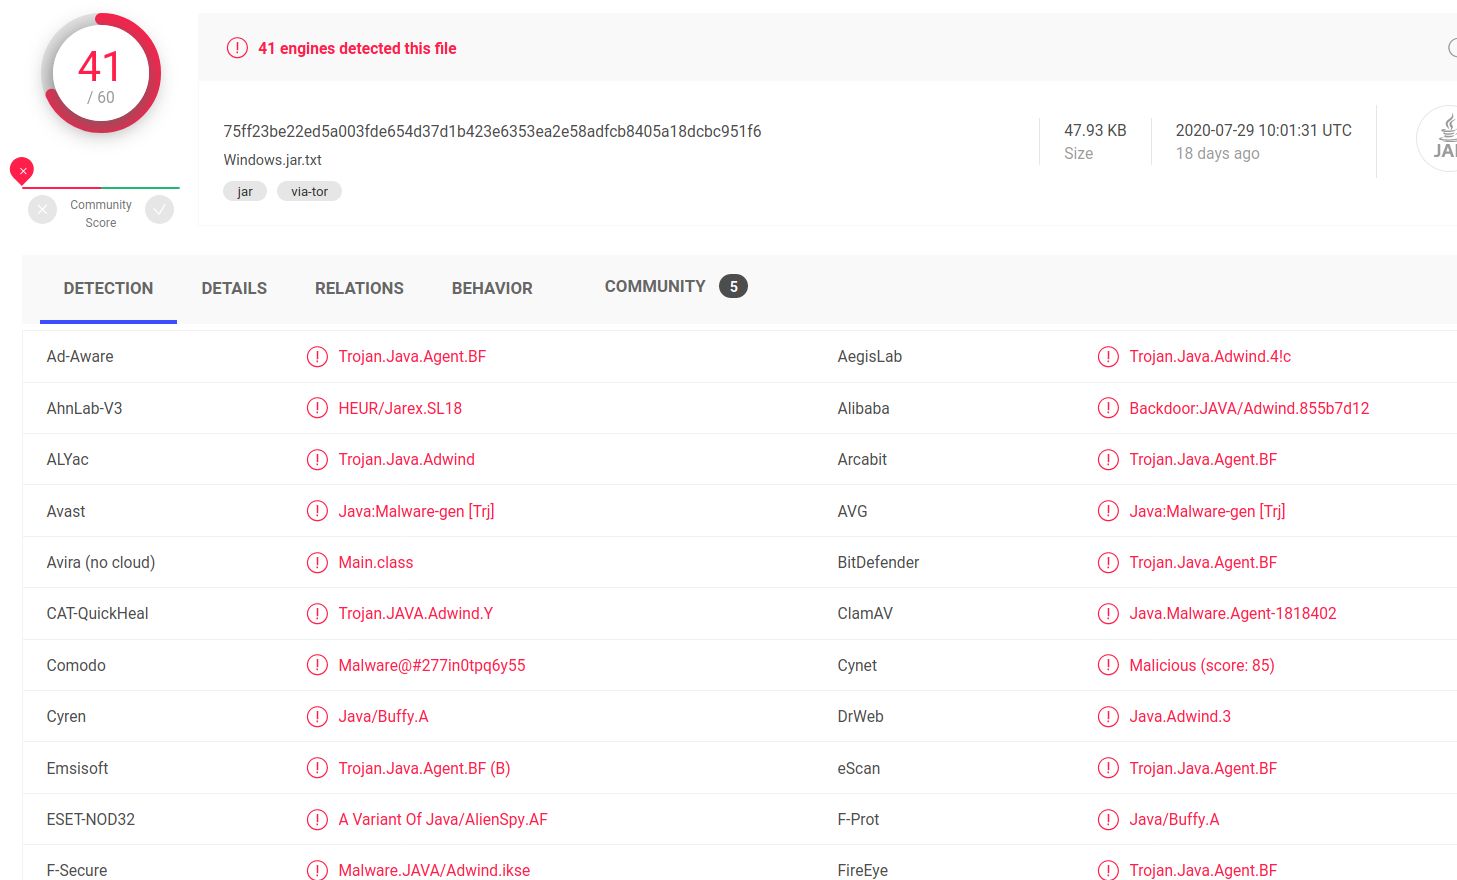
\includegraphics[width=0.5\linewidth]{purchase.png}

                    \\ ejecutando el analisis con el tercer binario pasa lo mismo que con el segundo 

                    \\ 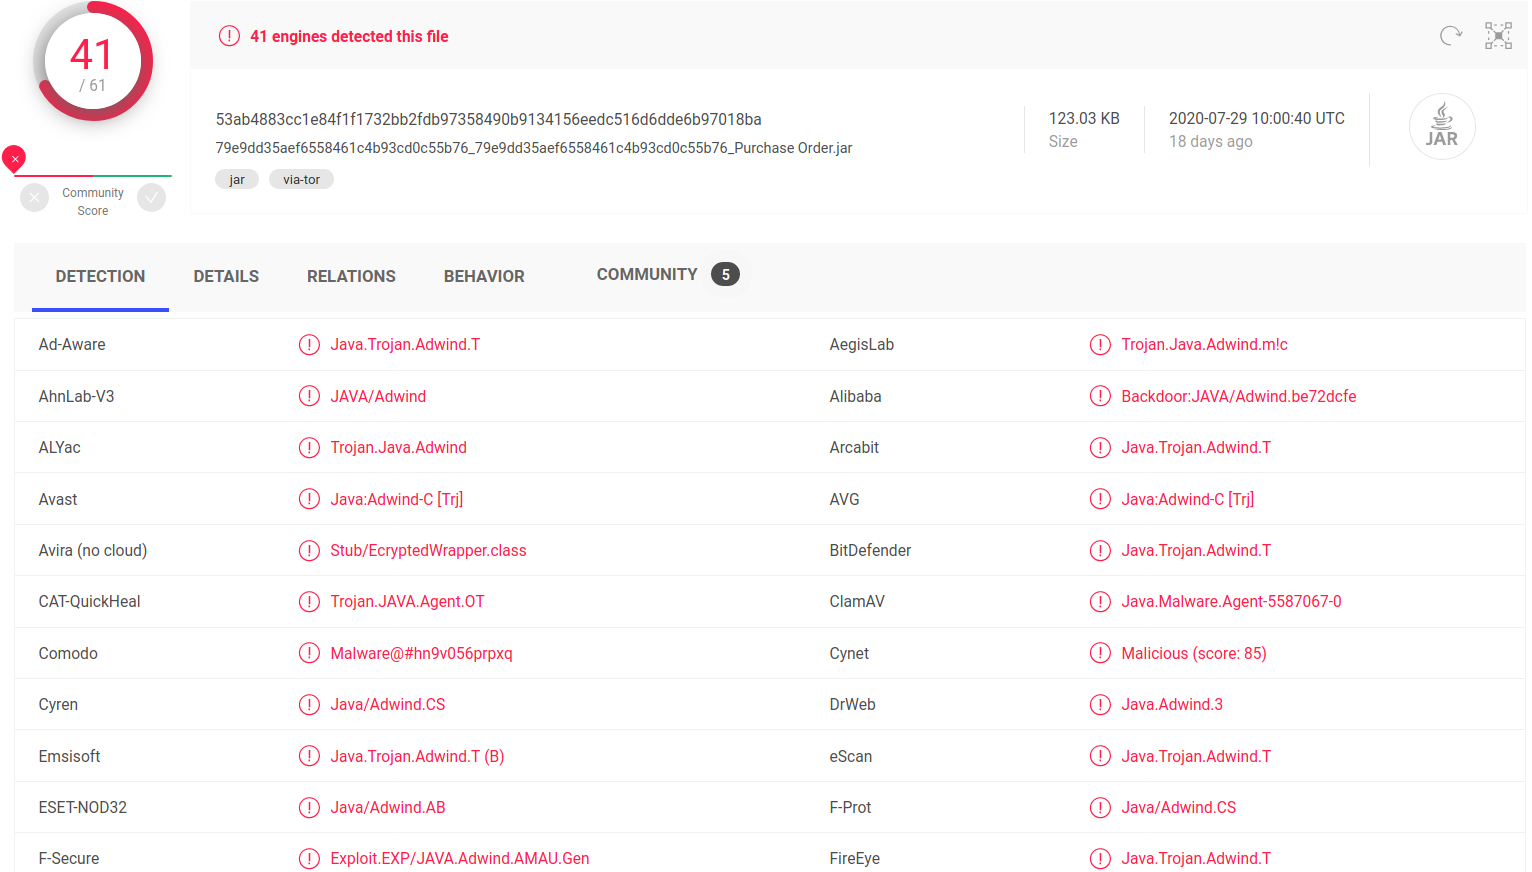
\includegraphics[width=0.5\linewidth]{purchase2.png}

                    \\ 

                \subsubsection{Analizando los archivos jar según sus caracteristicas individuales}

                    podemos ver los nombres que los diferentes antivirus ya le han asignado a estos archivos : 
                    \\ 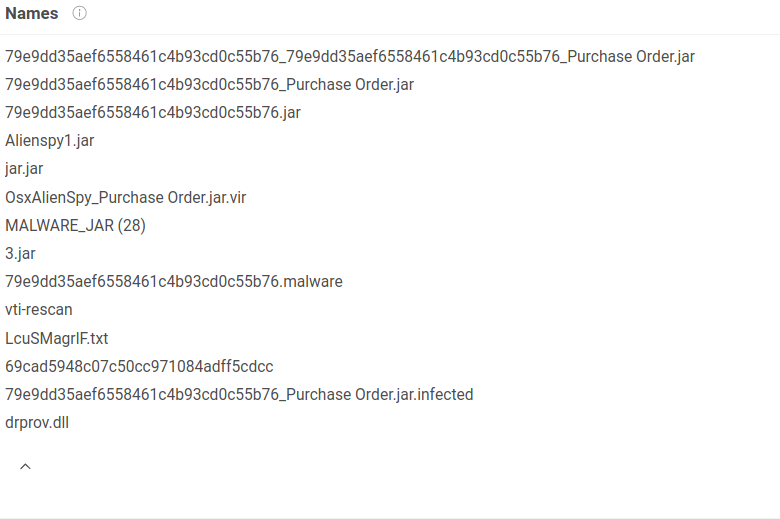
\includegraphics[width=0.5\linewidth]{names.png}
                    \\ tambien podemos ver los metadatos de los archivos file, nos muestra la siguiente información :
                    \\ 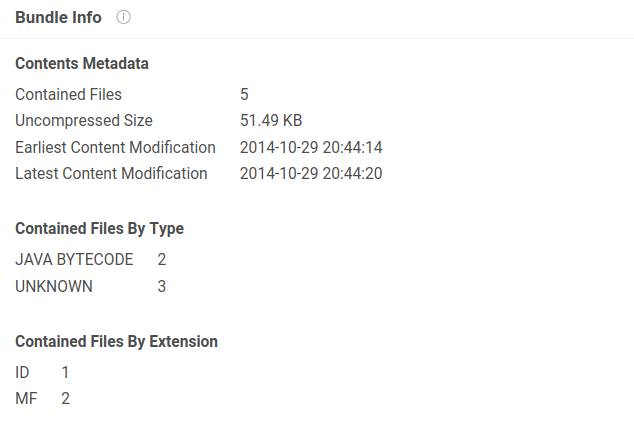
\includegraphics[width=0.8\linewidth]{metadata.png}
                    \\ en los metadatos se puede ver que el archivo fue creado
                    en 29 de diciembre de 2014 , el tamaño del archivo y la
                    cantidad de funciones que contiene , estos datos se pueden
                    ver en el binario de un archivo y son caracteres legibles,
                    sin embargo, existe una herramienta llamada exiftool que
                    los extrae automaticamente. 
                    
                    \\ También podemos ver que paquetes librerias de java está
                    importando el archivo: , la forma de hacer esto  
                    localmente es viendo los caracteres legibles del
                    binario mediante la herramienta strings. Esto puede ser de
                    vital imprtancia cuando queramos reversar el codigo del
                    malware en el futuro .
                    \\ 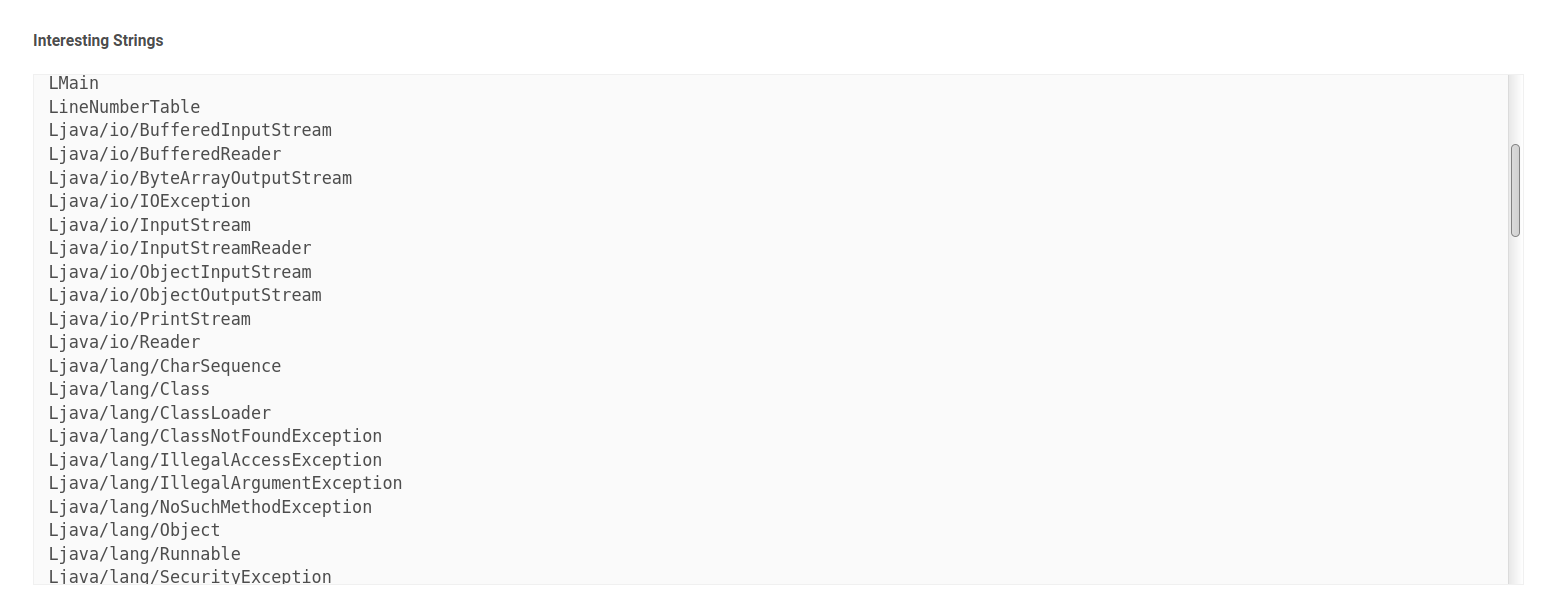
\includegraphics[width=0.9\linewidth]{librerias.png}
                    \\  

                    \subsubsection{Que otras cosas se pueden saber}
                        la razon principal por que elegí un troyano para hacer
                        este trabajo es porque esta clase de malware tiene que
                        conectarse a un servidor que maneja el atacante, es
                        posible ver los paquetes y mediante estos localizar el
                        servidor atacante, sin embargo , virustotal no hace
                        esto con los binarios tipo java, por lo que hacer esto
                        haria parte del analisis dinamico de maware (pues habria
                        que ejecutarlo o hacerle reversing)y no haria
                        parte de este trabajo :( .
                
           

    %=======================NOTES ENDS HERE===================%
    
    % bib stuff
    \nocite{*}
    \addtocontents{toc}{\protect\vspace{\beforebibskip}}
    \addcontentsline{toc}{section}{\refname}    
    \bibliographystyle{plain}
    \bibliography{../Bibliography}
\end{document}
